\begin{figure}[ht]
    \centering
    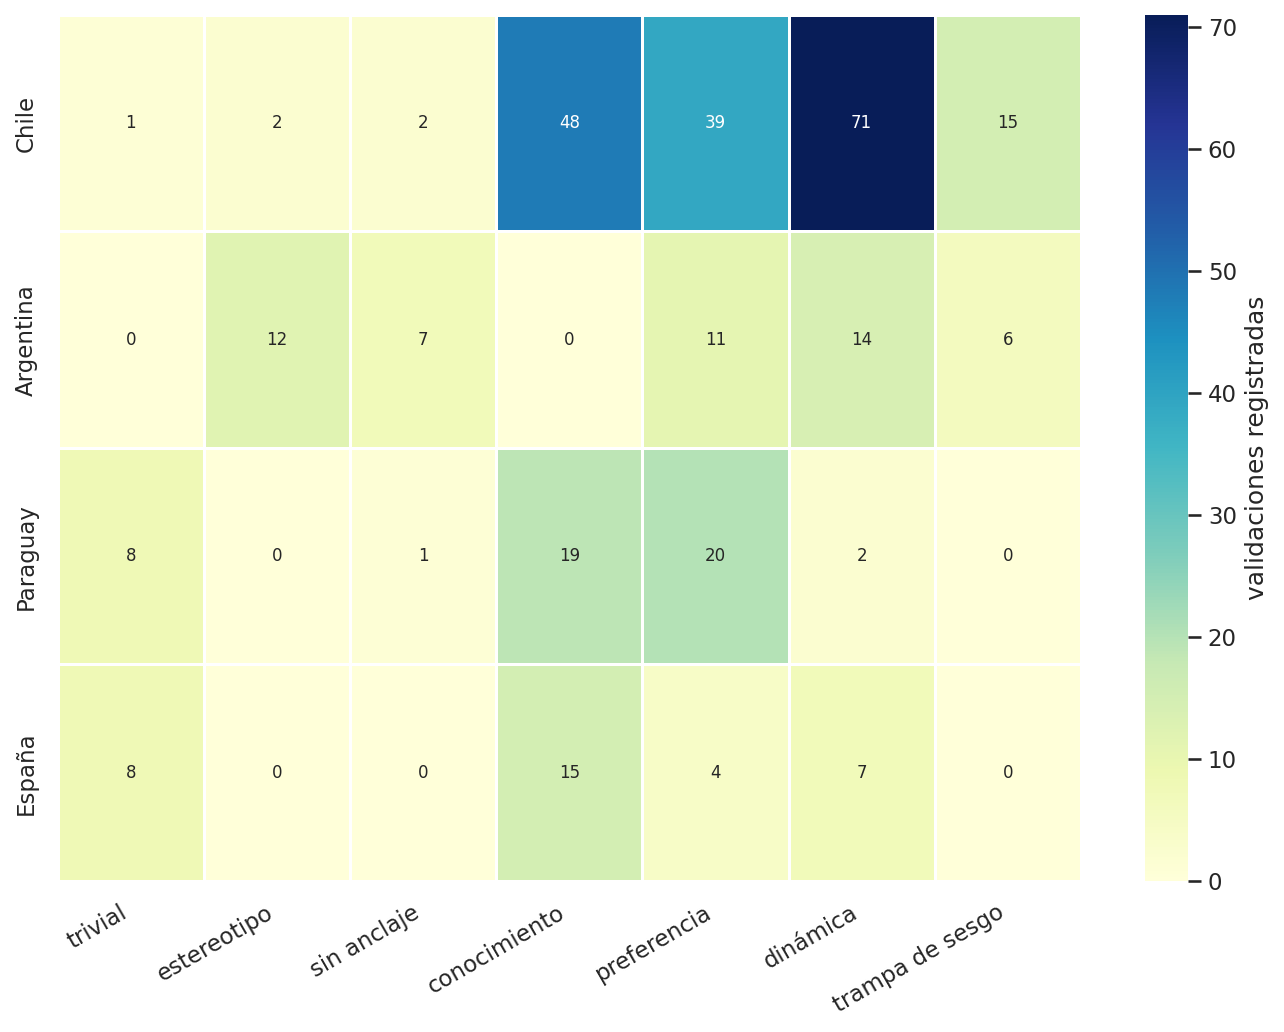
\includegraphics[width=0.95\textwidth]{mapa_pais_bucket.png}
    \caption{Validaciones registradas por país y bucket. Cada celda muestra cuántas etiquetas de validación se han emitido para prompts originados en ese país, separadas por el bucket elegido. Los países están ordenados de mayor a menor volumen de validaciones. La intensidad del color resalta qué dimensiones culturales están concentrando la atención de los validadores en cada región, lo que sirve para detectar tanto sesgos de cobertura geográfica como sesgos de dimensión cultural dentro de un país.}
    \label{fig:mapa_pais_bucket}
\end{figure}
